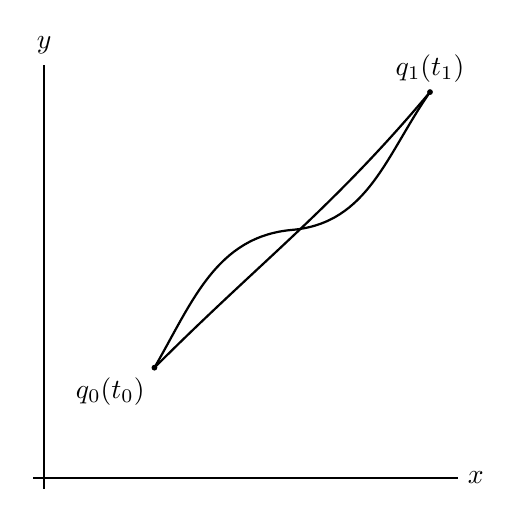
\begin{tikzpicture}[scale=0.7]

    % Draw the axes
    % The axes in the image cross slightly, so we extend them a bit past the origin
    \draw[thick] (-0.2, 0) -- (7.5, 0) node[right] {$x$} ;
    \draw[thick] (0, -0.2) -- (0, 7.5) node[above] {$y$};

    % Define the coordinates for the two points
    \coordinate (P1) at (2, 2);
    \coordinate (P2) at (7, 7);

    % Draw the bottom curve
    % It sags slightly below a straight line between the two points
    \draw[thick] (P1) to[out=45, in=230] (P2);

    % Draw the top curve
    % It has an S-shape, so we use an intermediate point to create the inflection
    \draw[thick] (P1) to[out=60, in=185] (4.5, 4.5) to[out=5, in=235] (P2);

    % Draw the points and their labels
    \fill (P1) circle (1.5pt) node[below left] {\(q_0(t_0)\)};
    \fill (P2) circle (1.5pt) node[above] {\(q_1(t_1)\)};

\end{tikzpicture}